\begin{abstract}
%
Machine learning has successfully leveraged modern data and provided computational solutions to innumerable real-world problems, including physical and biomedical discoveries. 
%
Currently, estimators could handle both scenarios with all samples available and situations requiring continuous updates.
%
However, there is still room for improvement on streaming algorithms based on batch decision trees and random forests, which are the leading methods in batch data tasks.
% tasks often require large sample sizes and continuing updates, which are both beyond the capacity of batch classifiers such as decision trees and random forests. 
%
% In contrast, streaming trees allow model fitting with new batches of samples without keeping the old data, thus saving computational resources and dealing with problems like out-of-distribution (OOD) inputs. 
In this paper, we explore the simplest partial fitting algorithm to extend batch trees and test our models: stream decision tree (\SDT) and stream decision forest (\SDF) on three classification tasks of varying complexities.
For reference, both existing streaming trees (Hoeffding trees and Mondrian forests) and batch estimators are included in the experiments.
% we benchmark two popular streaming tree estimators: Hoeffding trees (HTs) and Mondrian forests (MFs), and our own streaming tree and forest implementations in three classification tasks of varying complexities. 
%
In all three tasks, \SDF~consistently produces high accuracy, whereas existing estimators encounter space restraints and accuracy fluctuations. Thus, our streaming trees and forests show great potential for further improvements, which are good candidates for solving problems like distribution drift and transfer learning.
\end{abstract}

\section{Introduction}
\label{introduction}
In recent decades, machine learning methods continue to facilitate the utilization of modern data and make scientific progress in health care, technology, commerce, and more \citep{Jordan2015}. Their applications span across both fields with all samples ready to use and those with continuous data inputs, especially online data mining \citep{hoeffding}. 
Among all the methods, batch decision trees (DTs) and ensembles like random forests (RFs) are the leading strategies for batch tasks like classification, outperforming all others on real datasets and machine learning competitions \citep{Caruana2006-wp, Caruana2008-tb, JMLR:v15:delgado14a, Chen2016-fx}.
However, there lacks state-of-the-art streaming trees and forests on tasks having large sample sizes and requiring continual partial fitting.
Fitting datasets with larger sample sizes requires overwhelmingly more amounts of computational time and space. Moreover, different scenarios of streaming inputs would need flexible strategies for model updates \citep{abdulsalam07st}. This means that, for batch tree estimators like DT and RF, all sample data must be stored, and re-fitting everything is needed for each update \citep{Amit1997, breiman2001random}. 

Even with enough computational resources to do so, out-of-distribution (OOD) problems could undermine the validity of older data \citep{geisa2021theory}. In contrast, by partially fitting indefinite batches of new training samples, streaming trees can continuously update the tree structure without storing old data \citep{hoeffding, bifet2009adaptive, mondrian, JMLR:v11:ben-haim10a}. Furthermore, in forest ensembles, older trees could potentially be pruned to keep up with the current data distribution.
% many streaming tree algorithms have been developed to take advantage of data streams, including Hoeffding trees (HTs) and Mondrian forests (MFs) .
In this paper, we explore the simplest partial fitting method to extend a fitted decision tree and introduce our two streaming tree implementations: stream decision tree (\SDT) and stream decision forest (\SDF).
We test these estimators on three classification tasks with varying complexities. For reference, existing streaming trees like Hoeffding tree (HT) and Mondrian forest (MF), and batch estimators (DT and RF) are also included \citep{hoeffding, mondrian}. 

Among all streaming tree methods, our \SDF~produces consistently accurate results, whereas HT shows significant fluctuations in accuracy. MF, on the other hand, requires much more computational space and fails to perform consistently. Overall, \SDT~and \SDF~show good potentials for further improvements and would be better candidates for solving OOD problems \citep{geisa2021theory}. We can also use them to enhance transfer learning by adding new data to previously learned tasks \citep{vogelstein2021omnidirectional}.

\section{Methods} 
\label{methods}

\subsection{Algorithms}
% TODO describe THE ALGORITHMS in plain words in 1-2 paragraphs, including streaming trees, and forests.
% TODO include initialization
Both \SDT~and \SDF~are based on a customized fork of scikit-learn, which added the new \texttt{partial\_fit} function to \texttt{DecisionTreeClassifier} \citep{scikit-learn}. A \SDT~is initialized almost in the same way as a DT, where the tree fits the first training samples. The only difference is the input of predefined class labels ($cls$), as the first batch might not include all possible classes. After \SDT~is fitted, each arriving training set $\mathcal{D}_n$ would be sorted into leaf nodes marked as ``false roots'' (Algorithm \ref{alg:partial}). These ``false roots'' are then split and extended if the minimum sample size (two in default) is reached.

A \SDF, defined as \texttt{StreamDecisionForest}\footnote{\url{https://neurodata.io/sdtf/}}, is initialized as a collection of \SDT s (100 in default). As in Algorithm \ref{alg:sdf}, it partially fits the trees by randomly permuting the training batches given and limiting the number of features selected per split (``max-features'') to $\sqrt{d}$, where $d$ is the number of features. The predictions are generated by majority voting \citep{liaw2002classification, biau2008consistency, breiman2001random}. We benchmarked both \SDT~and \SDF~by training them with incremental batches of 100 random samples.

\begin{algorithm}[htb]
  \caption{Partially fit a \SDT~with one batch of training samples.}
\label{alg:partial}
\begin{algorithmic}[1]
  \Require 
  \Statex (1) $\mathcal{D}_n = (\mathbf{x},\mathbf{y}) \in \Real^{n \times p} \times \{1,\ldots, K\}^n$ \Comment{batch of training samples}
  \Statex (2) $cls$ \Comment{classes, required for first call}
  \Ensure 
  \Statex (1) $T$ \Comment{partially fitted tree}

\Function{\SDT.partial\_fit}{$\mathbf{x},\mathbf{y},cls$}
\If{tree is not fitted} 
  \State \Return \SDT.fit($\mathbf{x},\mathbf{y},cls$) \Comment{same as batch tree fitting except preset classes}
\EndIf
\For{each ($x$,$y$) in ($\mathbf{x},\mathbf{y}$)}
  \State find the leaf node $x$ would be sorted into \Comment{same as prediction}
  \State mark the node as a ``false root'' and associate ($x$,$y$) with it
\EndFor
\For{each ``false root''}
  \State update the node with associated samples
  \State split the node if satisfying minimum sample size
\EndFor

\State \Return $T$
\EndFunction 
\end{algorithmic}
\end{algorithm}

\begin{algorithm}[htb]
\caption{Partially fit a \SDF~with one batch of training samples.}
\label{alg:sdf}
\begin{algorithmic}[1]
  \Require
  \Statex (1) $\mathcal{D}_n = (\mathbf{x},\mathbf{y}) \in \Real^{n \times p} \times \{1,\ldots, K\}^n$ \Comment{batch of training samples}
  \Statex (2) $cls$ \Comment{classes, required for first call}
  \Ensure
  \Statex (1) $\mathbf{T}$ \Comment{partially fitted forest}
\Function{\SDF.partial\_fit}{$\mathbf{x},\mathbf{y},cls$}
\For{each $T$ in $\mathbf{T}$}
  \State ($\mathbf{x}^r,\mathbf{y}^r$) $\leftarrow$ randomize ($\mathbf{x},\mathbf{y}$)
  \State $T \leftarrow T$.partial\_fit($\mathbf{x}^r,\mathbf{y}^r,cls$) 
\EndFor
\State \Return $\mathbf{T}$
\EndFunction
\end{algorithmic}
\end{algorithm}

% \begin{algorithm}[htb]
% \caption{Partially fit a \CSF~with one batch of training samples.}
% \label{alg:csf}
% \begin{algorithmic}[1]
%   \Require
%   \Statex (1) $\mathcal{D}_n = (\mathbf{x},\mathbf{y}) \in \Real^{n \times p} \times \{1,\ldots, K\}^n$ \Comment{batch of training samples}
%   \Statex (2) $cls$ \Comment{classes, required for first call}
%   \Ensure
%   \Statex (1) $\mathbf{T}$ \Comment{partially fitted forest}
% \Function{\CSF.partial\_fit}{$\mathbf{x},\mathbf{y},cls$}
% \For{each $T$ in $\mathbf{T}$}
%   \State $T \leftarrow T$.partial\_fit($\mathbf{x},\mathbf{y},cls$) \Comment{partially fit existing trees}
% \EndFor
% \If{length of $\mathbf{T}$ is smaller than limit}
%   \State create a new $T'$
%   \State $T' \leftarrow T'$.partial\_fit($\mathbf{x},\mathbf{y},cls$)
%   \State add $T'$ to $\mathbf{T}$
% \EndIf
% \State \Return $\mathbf{T}$
% \EndFunction
% \end{algorithmic}
% \end{algorithm}

\subsection{Reference Algorithms}
For comparison with existing streaming trees, we selected two popular algorithms: HT and MF, and benchmarked them also with incremental batches of 100 random samples \citep{hoeffding, mondrian, OrpailleCC}. Open source code was used: \texttt{HoeffdingTreeClassifier} from the river package (BSD-3-Clause) and \texttt{MondrianForestClassifier} from the scikit-garden package (BSD-3-Clause) \citep{river, scikit-garden}. We set the max size of HT as 1,000 MB and used other hyperparameters as default. MF used the default 10 estimators to guarantee enough computational space.

For comparison with batch estimators, we included DT and RF: \texttt{DecisionTreeClassifier} and \texttt{RandomForestClassifier} from the original scikit-learn package (BSD-3-Clause) \citep{scikit-learn}. At each sample size, we trained both classifiers with all available samples, and all hyperparameters were kept as default. 

\subsection{Data}
We selected three datasets (Table \ref{table:data}) for the classification tasks: Splice-junction Gene Sequences (splice), Pen-Based Recognition of Handwritten Digits (pendigits), and CIFAR-10 \citep{splice, pendigits, cifar}. 
For the splice dataset, we randomly reserved 25\% of all genetic sequences for testing \citep{Rampone1998, Sarkar2020splice}. Each sequence contains 60 nucleotide codes, which are converted into numerical features by ordinal encoding: $A = 0.25$, $C = 0.50$, $G = 0.75$ and $T = 1.00$. All ambiguous nucleotides are represented by zero \citep{choong2017evaluation}. This task tests MF's performance on DNA data without feature engineering \citep{mondrian}. 
The pendigits dataset contains handwritten images represented by 16 pixel features, which are generated through spatial resampling \citep{Alimoglu96methodsof}.
The CIFAR-10 dataset contains RGB-colored images, each high-dimensional image represented by $32 \times 32 \times 3 = 3,072$ pixel features. We used the provided training and test sets for pendigits and CIFAR-10, and ran all tasks 10 times by randomizing the training sets. 

% TODO mention errorbars
\begin{table}[htb]
\centering
\begin{tabular}{ |c|c|c|c|c| } 
\hline
Name & No. features & No. classes & No. training samples & No. test samples \\
\hline
splice & 60 & 3 & 2,392 & 798 \\
\hline
pendigits & 16 & 10 & 7,494 & 3,498 \\
\hline
CIFAR-10 & 3,072 & 10 & 50,000 & 10,000 \\
\hline
\end{tabular}
\caption{Dataset attributes.}
\label{table:data}
\end{table}

\subsection{Evaluation Metrics}
Performance is evaluated by classification accuracy and training wall times. 
The training wall times calculate the fitting times for the given model without hyperparameter tuning. All estimators' fitting times are calculated by accumulating the training times of data batches, which account for batch estimators' refitting. We dot not report error bars as they are minimal.
All experiments were performed without parallelization on the same Microsoft Azure compute instance: a 6-core Standard\_NC6 (Intel Xeon E5-2690 v3) with 56 GB memory and 340 GB SSD storage.
\section{Results}
\label{results}

\begin{figure}[!htb]
\centering
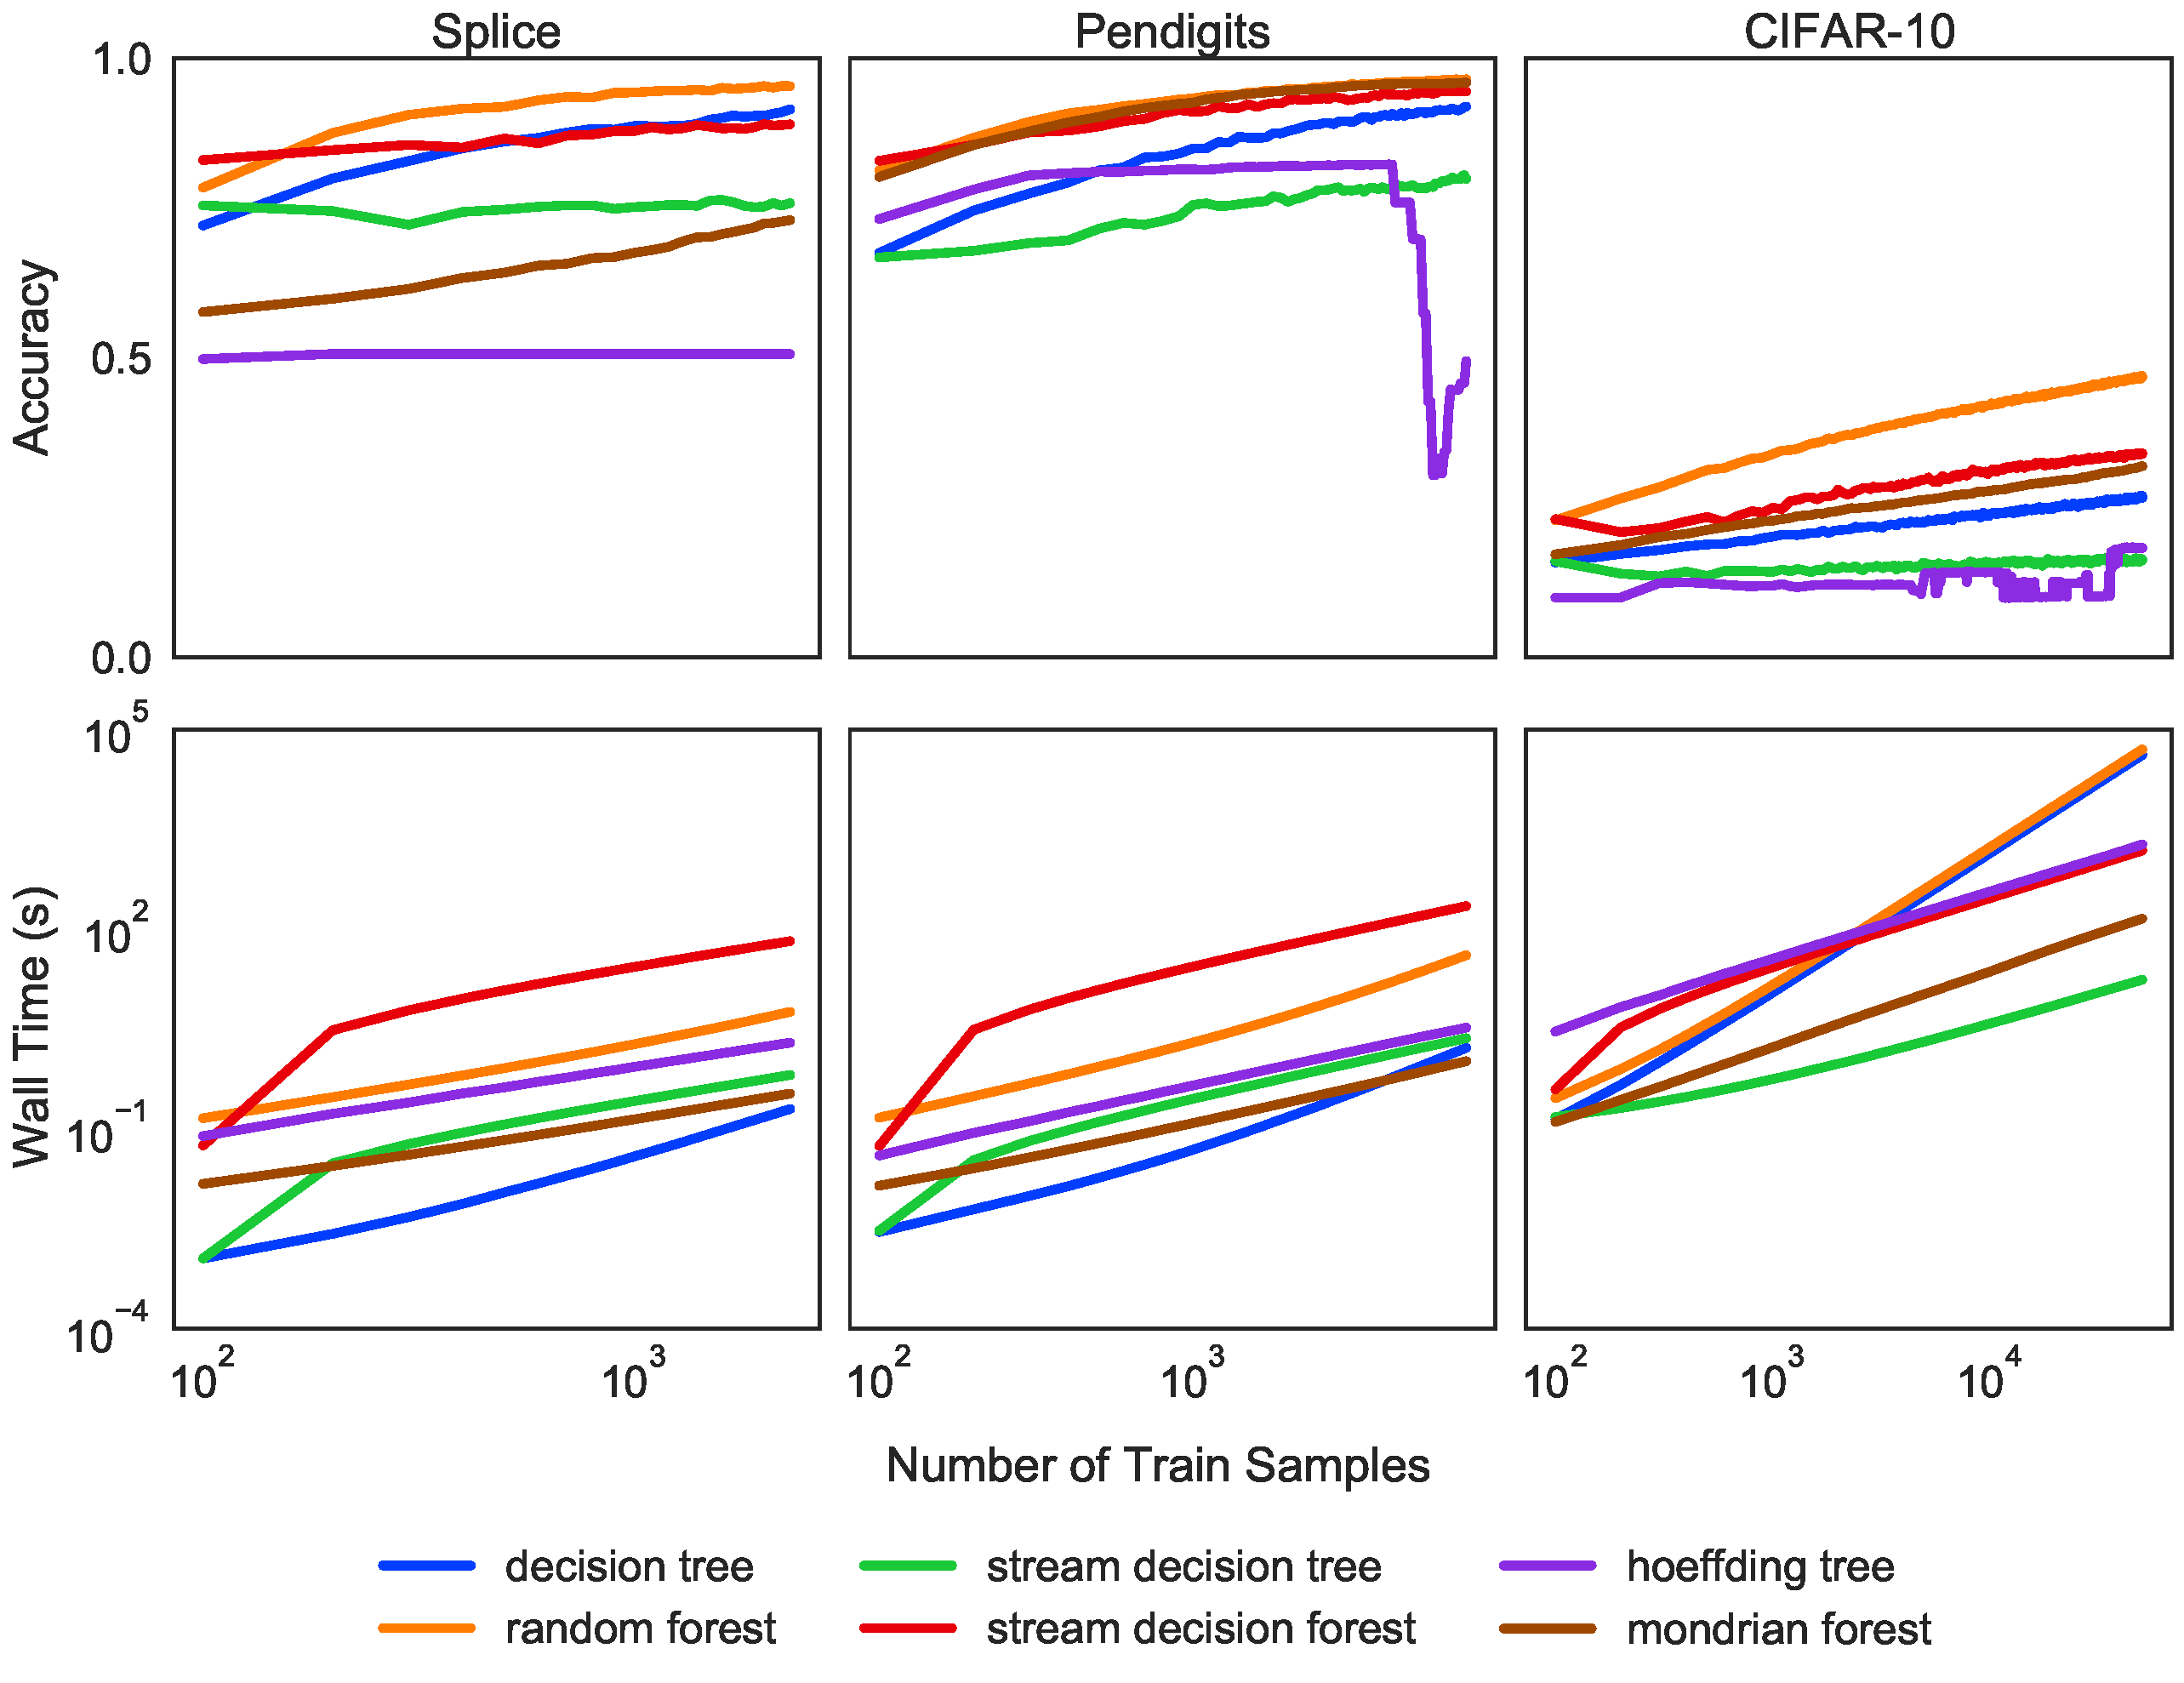
\includegraphics[width=1.0\textwidth]{visual.pdf}
  \caption{Multiclass classifications on splice \textbf{(left)}, pendigits \textbf{(center)}, and CIFAR-10 \textbf{(right)} datasets. 
  Each line represents averaged results from 10 randomized repetitions. At larger sample sizes, stream decision forests (\SDF) performs as well as or better than batch decision tree (DT) or other streaming estimators. Hoeffding tree (HT) either remains almost constant or experiences significant fluctuations in accuracy. Mondrian forest (MF) performs best in the pendigits task but only surpass HT in the splice task. Random forest (RF) achieves the highest accuracy in all tasks.
  For training wall times, cumulative fitting times are shown for all estimators, and two batch estimators' times include re-fitting at each sample size. \SDT~is the most efficient in the CIFAR-10 task. \SDF~takes longer times in the splice and pendigits tasks, but DT and RF overtake all streaming classifiers in the CIFAR-10 task. HT times increase significantly on the CIFAR-10 dataset.
  }
\label{fig:visual}
\end{figure}
% \vfil\eject

\subsection{Accuracy}
\SDF~tends to achieve high accuracy across all sample sizes and datasets, as compared to MF and HT (Figure \ref{fig:visual}, upper row). It performs as good as or better than DT. 
HT has the lowest accuracy when training on the splice dataset, which almost remains constant as sample size increases. It also experiences significant fluctuations when training on the pendigits and CIFAR-10 datasets. We speculate that this issue is caused by insufficient memory allocation, but increasing the max size could not alleviate the problem.
MF performs as good as RF in the pendigits task but only surpass HT on accuracy in the splice dataset. We find the difference as expected due to previous experiments, and the fluctuations could be attributed to the random partitions of Mondrian processes \citep{mondrian, roy2009mondrian}. The accuracy should be improved if feature engineering is implemented.
RF achieves the highest accuracy at most sample sizes.

\subsection{Training Wall Times}
\SDT~is the most efficient in the CIFAR-10 task. \SDF~takes longer training times in the two tasks with lower complexities, but DT and RF surpass all streaming estimators at larger sample sizes in the CIFAR-10 task (Figure \ref{fig:visual}, bottom row). The training times of HT increase significantly in the CIFAR-10 task, whereas MF's maintain more consistent trajectories. 
% Batch estimators (DT and RF) achieve efficient results and all training times increase with task complexities.

\section{Discussion}
\label{discussion}
Our implementations of streaming trees (\SDT~and \SDF) utilize the simplest partial fitting strategy (Algorithm \ref{alg:partial}), and achieve consistent and competent results in the three classification tasks. Also, \SDT~shows the most time efficiency on the high-dimensional CIFAR-10 dataset. By comparison, under a reasonable computational environment, we find memory overflow issues and performance fluctuations on two existing streaming estimators: HT and MF. This shows our methods' advantages on accuracy, stability and efficiency. 

Batch estimators could be more efficient and accurate if all samples are given at once, which would be nonetheless unlikely in real-world scenarios. In both our experiments and actual practices, batch decision trees and forests need to store all available data and re-fit them every time a new batch of samples comes in. Even by restricting the model updates with minimum batch samples, data storage would still cost significant computational resources. 

Overall, \SDT~and \SDF~show good potentials for further improvements. By optimizing our approaches, we intend to construct robust streaming estimators and add streaming trees to the scikit-learn package \citep{scikit-learn}. These models would be good candidates for solving OOD problems, and transfer learning could leverage the streaming capability to update existing tasks.